\documentclass[a4paper, czech]{article}

\usepackage[czech]{babel}
\usepackage{indentfirst}
\usepackage{graphicx}
\usepackage{float}
\usepackage[margin=1.5cm]{geometry}
\usepackage{booktabs}
\usepackage{amsmath}
\usepackage[dvipsnames]{xcolor}
\usepackage{multirow}
\usepackage{tabularray}
\usepackage{bold-extra}
\usepackage{circuitikz}
\usepackage{caption}
\usepackage{subcaption}
\usepackage[utf8]{inputenc}
\usepackage{array}

\begin{document}
\begin{table}[H]
    \centering
    \begin{tblr}{
        cell{1}{1} = {c = 2, r = 4}{c}, % Logo
        cell{1}{4} = {c = 3}{c}, % Předmět
        cell{2}{4} = {c = 3}{c}, % Jméno
        cell{3}{4} = {}{c}, % Ročník
        cell{3}{6} = {}{c}, % Studijní skupina
        cell{4}{4} = {}{c}, % Spolupracoval
        cell{4}{6} = {}{c}, % Mereno dne
        cell{5}{1} = {c = 2}{55mm}, % Kontroloval
        cell{5}{3} = {c = 2}{55mm}, % Hodnoceni
        cell{5}{5} = {c = 2}{55mm}, % Dne
        cell{6}{2} = {c = 5}{}, % Nazev ulohy
        cell{7}{1} = {}{c}, % Číslo úlohy
        cell{7}{2} = {c = 5}{c}, % Název úlohy
        vline{1,2,7} = {1.2pt},
        vline{3,5},
        hline{1,5,6,8} = {1.2pt},
        hline{2,3,4}
        }
        
\includegraphics{logo_fekt.png} & & \textsuperscript{Předmět} & \large \textbf{Měření v audiotechnice} \\
             & & \textsuperscript{Jméno} & \large \textbf{Karolína Šebestová} \\
             & & \textsuperscript{Ročník} & \large \textbf{3.} & \textsuperscript{Studijní skupina} & \large \textbf{St 14:00} \\
             & & \textsuperscript{Spolupracoval} & \large \textbf{Filip Kokavec} & \textsuperscript{Měřeno dne} & \large \textbf{13.11.2024} \\
        \textsuperscript{Kontroloval} & & \textsuperscript{Hodnocení} & & \textsuperscript{Dne} \\
        \textsuperscript{Číslo úlohy} & \textsuperscript{Název úlohy} \\
        \Large \textbf{7B} & \Large \textsc{\textbf{Měření přeslechů}} \\
    \end{tblr}
\end{table}

\section{Zadání}

\begin{itemize}
    \item Stanovte přeslech na blízkém konci rušeného vedení.
    \item Porovnejte kmitočtovou závislost přeslechů měřených vedení.
\end{itemize}

\section{Teoretický úvod}

Přeslech vzniká v důsledku induktivní, kapacitní či galvanické vazby mezi signálními vodiči.
Vazba může vzniknout také přes společnou zem jednotlivých vedení.
Jedná se os specifickou formu rušení, kdy signál pŘenášený jedním vedením ovlivňuje průběh signálu v jiném vedení.
Projevuje se u souběžně vedených vodičů

V důsledku útlumu a rušení pak dochází ke zkreslení přenášeného signálu, které u datových přenosů v konečné podobě projevuje příjmem jiných dat, než jaké byly skutečně vyslány.

Podle místa na rušeném vedení rozlišujeme přeslech signálu na blízkém a vzdáleném konci, viz obr: Vznik přeslechu na Blízkém (NEXT) a vzdáleném (FEXT) konci vedení. Jedná se o veličinu, která vyjadřuje, kolik rušivého signálu se dostává z jednoho páru do jiného páru vedení. Při měření vlastností vedení je další důležitou veličinou útlum vlivem ztrát na vedení. 

\begin{figure}[H]
    \centering
    \begin{circuitikz}[european]
        \draw (0,0) to[R, l=$Z_g$] (2,0) node[ocirc, scale=2](gen1){} to[short] +(1,0) node[ocirc, scale=2](pripravek1){}
        (pripravek1) to[R, l=$Z_{p/2}$] +(2,0) node[ocirc, scale=2](Z011){};
        \draw[ultra thick, red] (Z011) to[short, l=$Z_{01}$] +(5,0) coordinate(Z012);
        \draw[ultra thick, red] (Z011) +(0,-2) coordinate(Z013) to[short] +(5,-2) coordinate(Z014);
        \draw (Z012) node[ocirc, scale=2](Z012){}
        (Z013) node[ocirc, scale=2](Z013){}
        (Z014) node[ocirc, scale=2](Z014){};
        \draw (Z013) to[R, l_=$Z_{p/2}$] +(-2,0) node[ocirc, scale=2](pripravek2){}
        (pripravek2) to[short] +(-1,0) node[ocirc, scale=2](gen2){}
        (gen2) to[short] +(-2,0) to[rmeter, t=$U_g$] (0,0);
        \draw (Z012) to[short] +(1,0) to[R, l=$Z_{out1}$] +(1,-2)
        (Z014) to[] +(1,0);

        \draw[ultra thick, blue] (Z013) +(0,-2) coordinate(Z111) to[short, l=$Z_{02}$] +(5,-2) coordinate(Z112);
        \draw[ultra thick, blue] (Z111) +(0,-2) coordinate(Z113) to[short] +(5,-2) coordinate(Z114);
        \draw (Z112) node[ocirc, scale=2, label={Vzdálený konec}](Z112){}
        (Z113) node[ocirc, scale=2](Z113){}
        (Z114) node[ocirc, scale=2](Z114){}
        (Z111) node[ocirc, scale=2, label={Blízký konec}](Z111){};

        \draw (Z111) to[] +(-1,0) to[R, l=$Z_{in2}$] +(-1,-2) to (Z113);
        \draw (Z112) to[] +(1,0) to[R, l=$Z_{out2}$] +(1,-2) to (Z113);

        \draw[-{Straight Barb[angle'=60, scale=2]}, blue] (Z111) +(0,-0.25) to[short, l=$U_{NEXT}$] +(0,-1.75);
        \draw[-{Straight Barb[angle'=60, scale=2]}, blue] (Z011) +(0,-0.25) to[short, l=$U_{in}$] +(0,-1.75);
        \draw[-{Straight Barb[angle'=60, scale=2]}, blue] (Z012) +(0,-0.25) to[short, l_=$U_{out}$] +(0,-1.75);

        \draw (7.5,-1) node[]{Rušící vedení};
        \draw (7.5,-5) node[]{Rušené vedení};

        \draw [densely dashed] (gen1) to (gen2) to +(0,-1) to (-1,-3) to (-1,1) to (2,1) to (gen1);
        \draw [densely dashed] (pripravek1) to (pripravek2) to (3,-7) to (12.5,-7) to (12.5,1) to (3,1) to (pripravek1);

        \draw (0.5,-2.5) node[]{Generátor};
        \draw (7.5,-6.5) node[]{Generátor};
    \end{circuitikz}
    \caption{Měření přeslechu na blízkém (NEXT) konci vedení.}
\end{figure}

\section{Výsledky měření}

\subsection{Tabulky}

\begin{table}[H]
    \catcode`\-=12
    \centering
    \caption{Měření přeslechů na blízkém konci (NEXT) souběžného vedení}
    \begin{tabular}{r>{\color{BrickRed}}c>{\color{BrickRed}}c>{\color{BrickRed}}c>{\color{OliveGreen}}c>{\color{OliveGreen}}c>{\color{OliveGreen}}c>{\color{BlueViolet}}c>{\color{BlueViolet}}c>{\color{BlueViolet}}c}
        \toprule
        \multirow{2}{*}{} & \multicolumn{3}{>{\color{BrickRed}}c}{\textit{Reproduktorová dvojlinka}} & \multicolumn{3}{>{\color{OliveGreen}}c}{\textit{UTP kat. 6}}         & \multicolumn{3}{>{\color{BlueViolet}}c}{\textit{S-STP kat. 7}}               \\
                        & \multicolumn{3}{>{\color{BrickRed}}c}{Dvojlinka}                & \multicolumn{3}{>{\color{OliveGreen}}c}{Kroucená dvojlinka} & \multicolumn{3}{>{\color{BlueViolet}}c}{Stíněná kroucená dvojlinka} \\
        \cmidrule(rl){2-4}
        \cmidrule(rl){5-7}
        \cmidrule(rl){8-10}
        \multicolumn{1}{c}{$f$}                 & $U_\text{in}$          & $U_\text{out}$          & $U_\text{NEXT}$         & $U_\text{in}$          & $U_\text{out}$          & $U_\text{NEXT}$       & $U_\text{in}$          & $U_\text{out}$          & $U_\text{NEXT}$         \\
        \cmidrule(rl){1-1}
        \cmidrule(rl){2-2}
        \cmidrule(rl){3-3}
        \cmidrule(rl){4-4}
        \cmidrule(rl){5-5}
        \cmidrule(rl){6-6}
        \cmidrule(rl){7-7}
        \cmidrule(rl){8-8}
        \cmidrule(rl){9-9}
        \cmidrule(rl){10-10}
        \multicolumn{1}{c}{MHz}               & V            & V             & mV            & V          & V           & mV          & V             & V              & mV            \\
        \cmidrule(rl){1-10}
        0,01              & 2            & 2,01          & 2,93          & 2          & 1,95        & 2,24        & 2             & 1,95           & 3,31          \\
        0,02              & 2            & 2,01          & 4,82          & 2          & 1,95        & 3,12        & 2             & 1,95           & 3,11          \\
        0,05              & 2            & 2,01          & 10,6          & 2          & 1,95        & 6,60        & 2             & 1,94           & 3,06          \\
        0,07              & 2            & 2,01          & 15,5          & 2          & 1,94        & 9,00        & 2             & 1,93           & 3,04          \\
        0,1               & 2            & 2,03          & 21,6          & 2          & 1,93        & 12,7        & 2             & 1,93           & 2,93          \\
        0,2               & 2            & 2,06          & 42,5          & 2          & 1,92        & 25,6        & 2             & 1,90           & 2,65          \\
        0,5               & 2            & 2,29          & 127           & 2          & 1,90        & 68,0        & 2             & 1,86           & 2,15          \\
        0,7               & 2            & 2,63          & 234           & 2          & 1,90        & 102         & 2             & 1,86           & 2,00          \\
        1                 & 2            & 3,81          & 620           & 2          & 1,88        & 160         & 2             & 1,85           & 1,88          \\
        5                 & 2            & 4,50          & 930           & 2          & 1,83        & 16,5        & 2             & 1,75           & 2,01          \\
        7                 & 2            & 1,56          & 126           & 2          & 1,89        & 670         & 2             & 1,96           & 2,71          \\
        10                & 2            & 1,90          & 360           & 2          & 1,77        & 44,0        & 2             & 1,53           & 2,15          \\
        \bottomrule
    \end{tabular}
\end{table}

\begin{table}[H]
    \catcode`\-=12
    \centering
    \caption{Vypočtené hodnoty $A$, $NEXT$ a $ACR_\text{N}$ pro jednotlivé typy dvojlinek}
    \begin{tabular}{r>{\color{BrickRed}}c>{\color{BrickRed}}c>{\color{BrickRed}}c>{\color{OliveGreen}}c>{\color{OliveGreen}}c>{\color{OliveGreen}}c>{\color{BlueViolet}}c>{\color{BlueViolet}}c>{\color{BlueViolet}}c}
        \toprule
        \multirow{2}{*}{} & \multicolumn{3}{>{\color{BrickRed}}c}{\textit{Reproduktorová dvojlinka}} & \multicolumn{3}{>{\color{OliveGreen}}c}{\textit{UTP kat. 6}}         & \multicolumn{3}{>{\color{BlueViolet}}c}{\textit{S-STP kat. 7}}               \\
                        & \multicolumn{3}{>{\color{BrickRed}}c}{Dvojlinka}                & \multicolumn{3}{>{\color{OliveGreen}}c}{Kroucená dvojlinka} & \multicolumn{3}{>{\color{BlueViolet}}c}{Stíněná kroucená dvojlinka} \\
        \cmidrule(rl){2-4}
        \cmidrule(rl){5-7}
        \cmidrule(rl){8-10}
        \multicolumn{1}{c}{$f$}                 & $A$          & $NEXT$          & $ACR_\text{N}$         & $A$          & $NEXT$          & $ACR_\text{N}$       & $A$          & $NEXT$          & $ACR_\text{N}$         \\
        \cmidrule(rl){1-1}
        \cmidrule(rl){2-2}
        \cmidrule(rl){3-3}
        \cmidrule(rl){4-4}
        \cmidrule(rl){5-5}
        \cmidrule(rl){6-6}
        \cmidrule(rl){7-7}
        \cmidrule(rl){8-8}
        \cmidrule(rl){9-9}
        \cmidrule(rl){10-10}
        \multicolumn{1}{c}{MHz}               & dB            & dB             & dB            & dB            & dB             & dB          & dB            & dB             & dB            \\
        \cmidrule(rl){1-10}
        0,01              & -0,043         & 56,68        & 56,73        & 0,220       & 59,02       & 58,80      & 0,220          & 55,62          & 55,40        \\
        0,02              & -0,043         & 52,36        & 52,40        & 0,220       & 56,14       & 55,92      & 0,220          & 56,17          & 55,95        \\
        0,05              & -0,043         & 45,51        & 45,56        & 0,220       & 49,63       & 49,41      & 0,265          & 56,31          & 56,04        \\
        0,07              & -0,043         & 42,21        & 42,26        & 0,265       & 46,94       & 46,67      & 0,309          & 56,36          & 56,05        \\
        0,1               & -0,129         & 39,33        & 39,46        & 0,309       & 43,94       & 43,64      & 0,309          & 56,68          & 56,37        \\
        0,2               & -0,257         & 33,45        & 33,71        & 0,355       & 37,86       & 37,50      & 0,446          & 57,56          & 57,11        \\
        0,5               & -1,176         & 23,94        & 25,12        & 0,446       & 29,37       & 28,92      & 0,630          & 59,37          & 58,74        \\
        0,7               & -2,379         & 18,64        & 21,01        & 0,446       & 25,85       & 25,40      & 0,630          & 60,00          & 59,37        \\
        1                 & -5,598         & 10,17        & 15,77        & 0,537       & 21,94       & 21,40      & 0,677          & 60,54          & 59,86        \\
        5                 & -7,044         & 6,651        & 13,69        & 0,772       & 41,67       & 40,90      & 1,160          & 59,96          & 58,80        \\
        7                 & 2,158          & 24,01        & 21,86        & 0,491       & 9,499       & 9,008      & 0,175          & 57,36          & 57,19        \\
        10                & 0,446          & 14,89        & 14,45        & 1,061       & 33,15       & 32,09      & 2,327          & 59,37          & 57,05        \\
        \bottomrule
    \end{tabular}
\end{table}

\subsection{Grafy}

\begin{figure}[H]
    \centering
    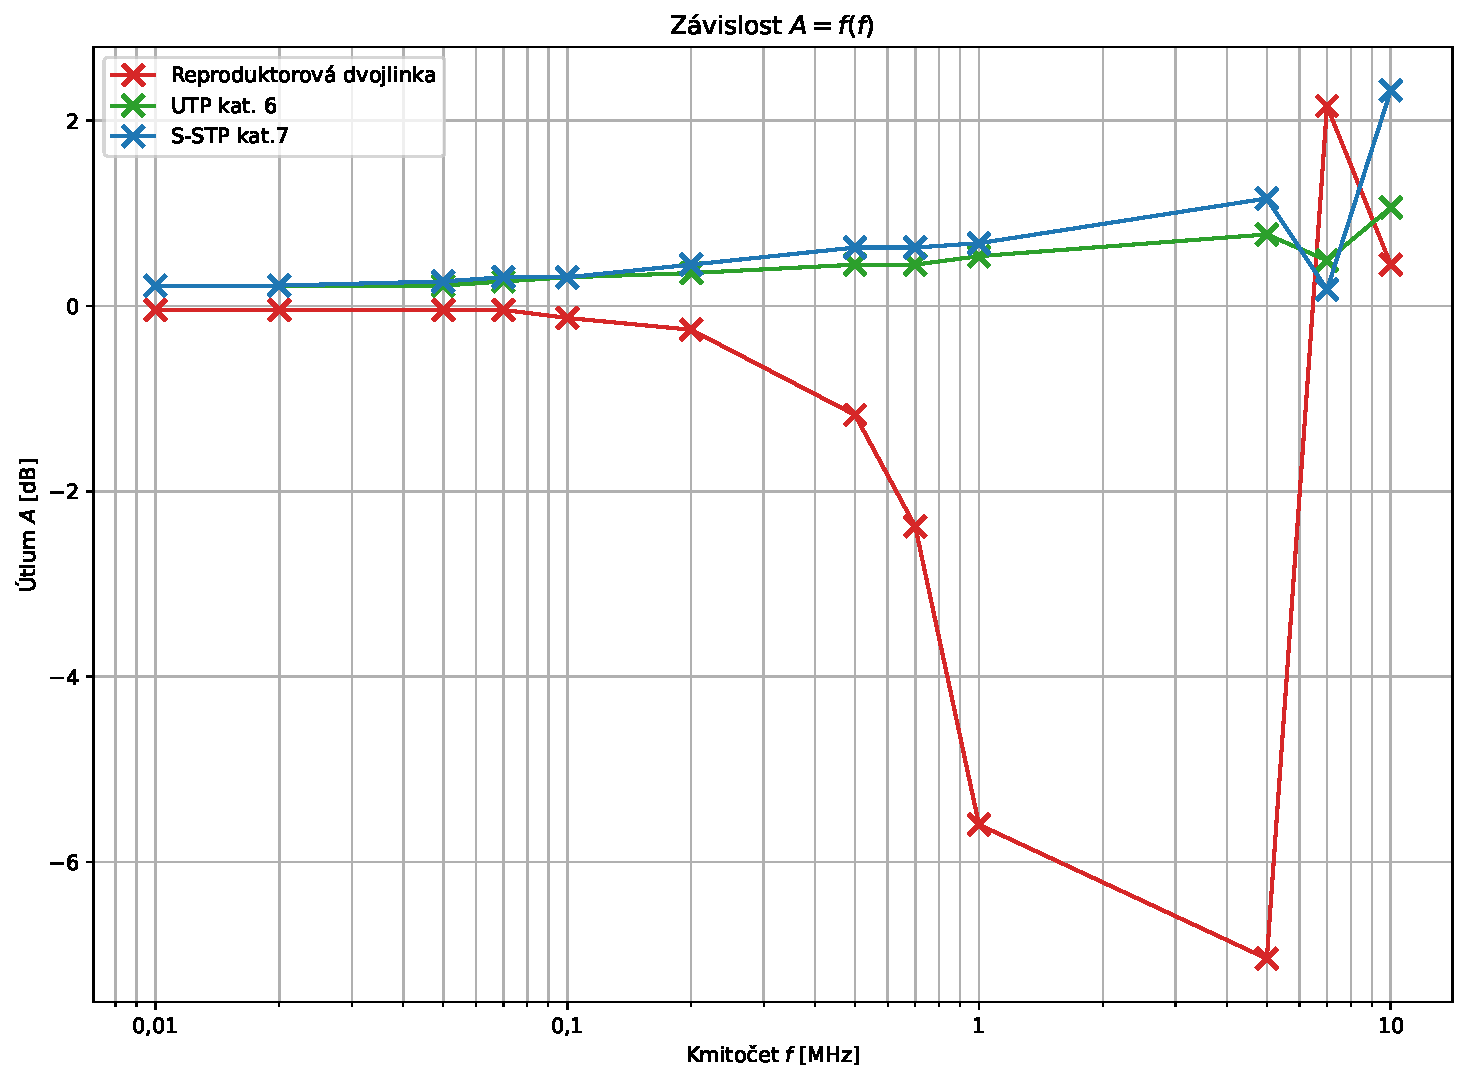
\includegraphics[width=0.8\textwidth]{grafy/graf1.pdf}
    \caption{Útlum vlivem ztrát $A$ v závislosti na kmitočtu $f$}
\end{figure}

\begin{figure}[H]
    \centering
    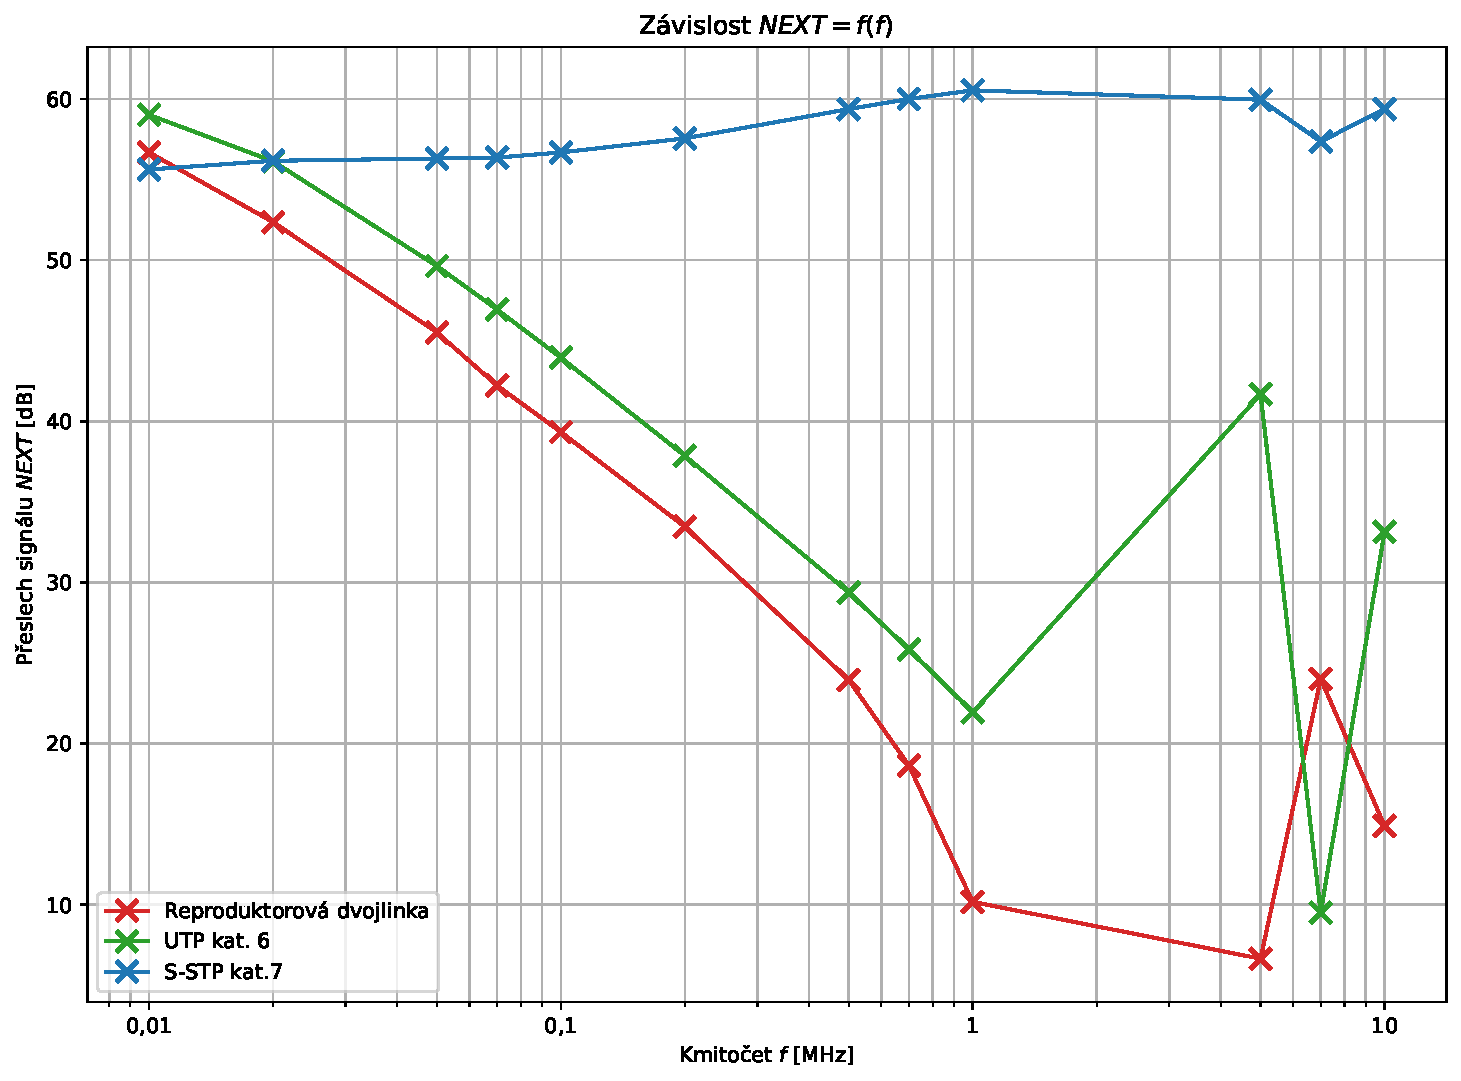
\includegraphics[width=0.8\textwidth]{grafy/graf2.pdf}
    \caption{Přeslech signálu $NEXT$ v závislosti na kmitočtu $f$}
\end{figure}

\begin{figure}[H]
    \centering
    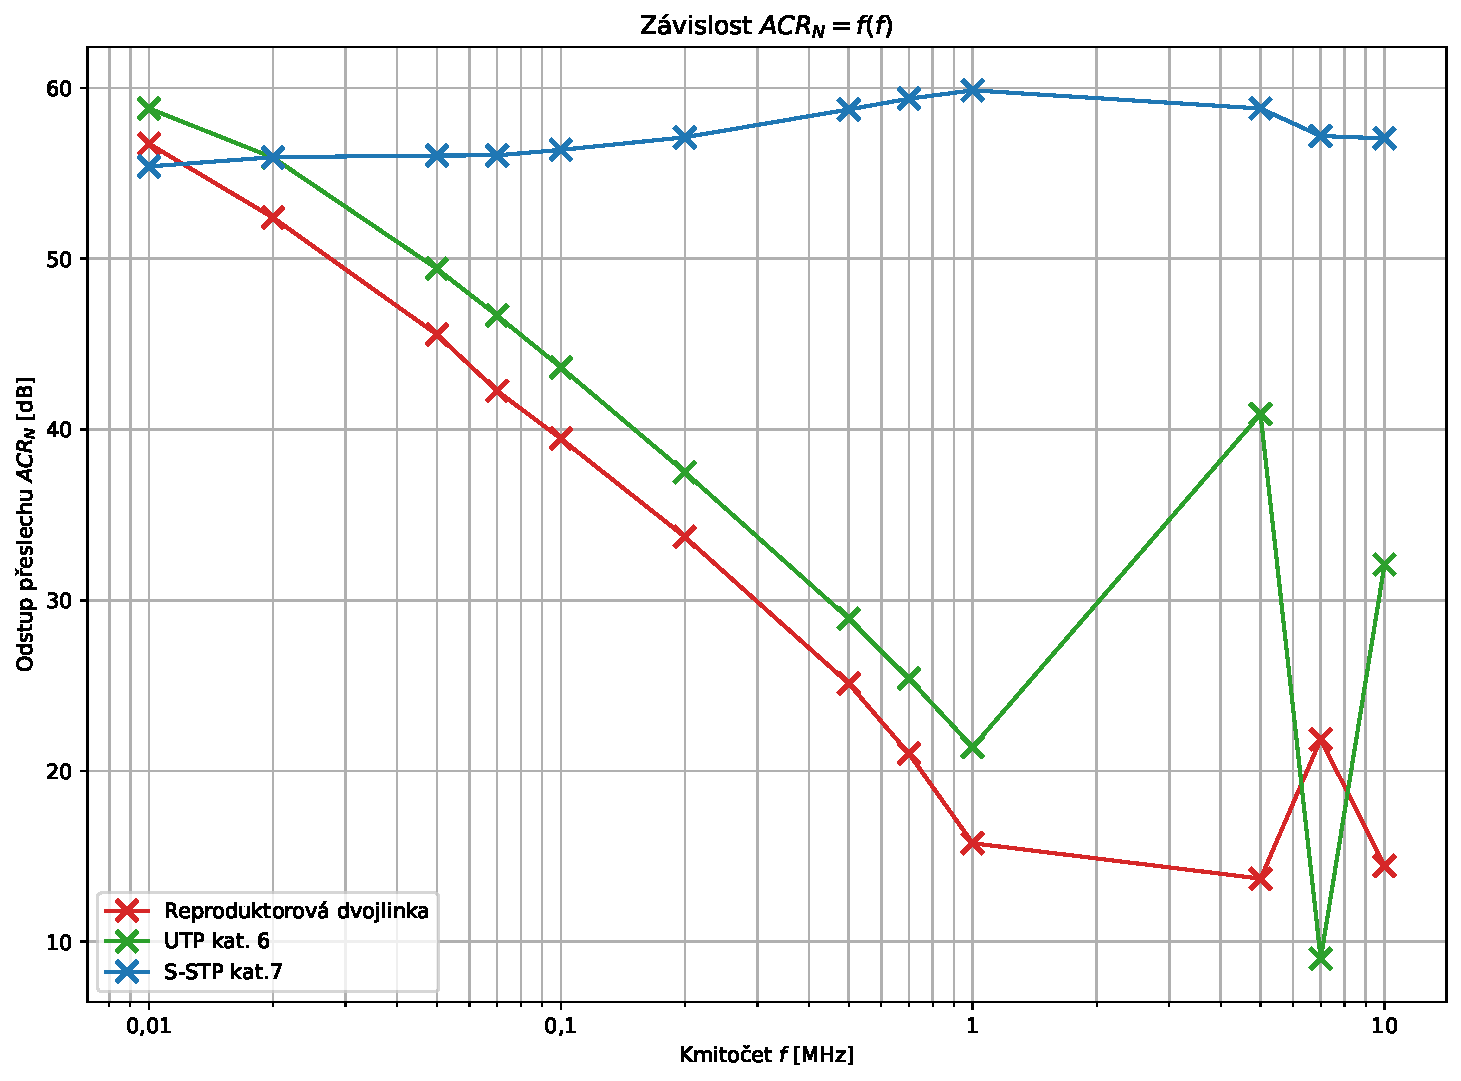
\includegraphics[width=0.8\textwidth]{grafy/graf3.pdf}
    \caption{Odstup přeslechu $ACR_\text{N}$ v závislosti na kmitočtu $f$}
\end{figure}

\subsection{Příklady výpočtu}

\begin{enumerate}
    \item Útlum vlivem ztrát na vedení
    \begin{multline*}
        A = \textcolor{teal}{20 \cdot \log \frac{\left|U_\text{in}\right|}{\left|U_\text{out}\right|}} = 20 \cdot \log \frac{\left|2\,\text{V}\right|}{\left|2,01\,\text{V}\right|} = \underline{\underline{-0,043\,\text{dB}}} \hfill
    \end{multline*}
    \item Přeslech signálu na blízkém konci
    \begin{multline*}
        NEXT = \textcolor{teal}{20 \cdot \log \frac{\left|U_\text{in}\right|}{\left|U_\text{NEXT}\right|} + 10 \cdot \log \frac{\left|Z_{01}\right|}{\left|Z_{02}\right|}} = 20 \cdot \log \frac{\left|2\,\text{V}\right|}{\left|2,93 \cdot 10^{-3}\,\text{V}\right|} = \underline{\underline{56,68\,\text{dB}}} \hfill
    \end{multline*}
    \item Odstup přeslechu na blízkém konci
    \begin{multline*}
        ACR_\text{N} = \textcolor{teal}{NEXT - A} = 56,68\,\text{dB} - (-0,043\,\text{dB}) =\underline{\underline{56,73\,\text{dB}}} \hfill
    \end{multline*}
\end{enumerate}

\section{Seznam použitých přístrojů}

\begin{itemize}
    \item Digitální osciloskop Agilent DSO-X 2004A, v.č. MY50513107
    \item Digitální signálový generátor Agilent 33250A, v.č. MY40028984
\end{itemize}

\section{Závěr}

Cílem měření bylo stanovit přeslech na blízkém konci rušivého vedení a porovnat kmitočtovou závislost přeslechů měřených vedení.

Z grafu prvního grafu je možné odečíst, že největších hodnot útlumu vlivem ztrát $A$ nabývá reproduktorová dvojlinka. Obě kroucené dvojlinky vykazují značně lepší hodnoty.

Z grafu druhého je možné odečíst, že při měření útlumu přeslechu $NEXT$ nestíněné dvojlinky značně strádají. Neboť stínění je právě to, co přeslechu zabraňuje.

Z našeho měření jasně vyplývá, že nejvhodnějším typem dvojlinky s ohledem na měřené parametry pro přenášení signálu od 0,01 do 10 MHz je stíněná dvojlinka S-STP kat. 7, avšak pokud vezmeme v úvahu, že pro úspěšný přenos dat musí být hodnota $ACR_N$ alespoň 10 dB, tak je jasné, že všechny dvojlinky tuto podmínku splňují. 

\end{document}